\chapter{图像生成模型}
\label{cha:sysu-thesis-contents-format-requirement}
图像生成模型的核心挑战在于:如何将简单分布(如高斯分布)映射到复杂的数据分布(图像),这需要复杂的深度学习技术。
在生成建模过程中,深度神经网络用于学习概率分布的表示,从而将简单的输入转换为复杂输出。模型将使用图像集作为训练集(如人脸照片,掌静脉图像),无监督地捕捉数据内在规律。
使得生成结果在风格、内容上与训练集一致。

然而,无监督学习成为了生成模型的训练难点。
在分类或检测任务中,训练集本身会给出标签(标准答案),引导模型的输出向标准答案靠拢。
比如图像分类任务,训练集会给出每一幅图像的类别;对于人脸验证任务,训练集会给出两张人脸照片是不是同一个人;
对于目标检测任务,训练集会给出目标的具体位置编码。

生成任务无标签(没有标准答案),缺乏监督信号,高度依赖数据分布本身的统计特性。
常见的优秀生成模型包括对抗训练GAN、变分推断VAE和概率建模Diffusion,具有更高的图像生成质量。

\section{生成对抗网络}
生成式对抗网络(generative adversarial networks,GAN)是一种深度学习模型,由Ian Goodfellow等人于2014年提出\cite{goodfellow2014generative}。
在GAN模型提出以前,生成模型主要基于概率图模型、隐变量模型等方法:如概率生成模型和自动
编码器。这些方法在生成样本时面临着训练困难和生成样本质量低下的问题。
生成对抗网络引入了对抗博弈的思想,通过对抗训练的方式,同时训练生成器和判别器,实现生成高质量样本的能力。

作为基于博弈思想的生成模型,GAN主要由生成器与判别器两部分组成。核心思想是通过让生成器生成逼真的样本,以欺骗判别器来提高生成器的能力。
生成器接受一个随机向量$\mathbf{z}$作为输入,并通过一系列的转换将其映射到数据空间中。判别器则负责对生成器生成的样本和真实样本进行区分。
通过不断迭代训练,直到对抗达到均衡,损失收敛时,生成器能够生成高度逼真的样本,在视觉上几乎无法与真实数据区分开来,实现数据生成的任务。
同时,我们也得到了一个优质的判别器进行分类任务。

在\autoref{fig:GAN}中给出了GAN的基本框架,其中$x$表示需要学习的真实数据,服从分布$P_{data}(x)$;
$z$表示随机输入的噪声,服从分布$P_{seed}(z)$;$G(z;\theta)$和$D(x;\phi)$分别表示生成网络和判别网络。
\begin{figure}[!htbp]
    \centering
    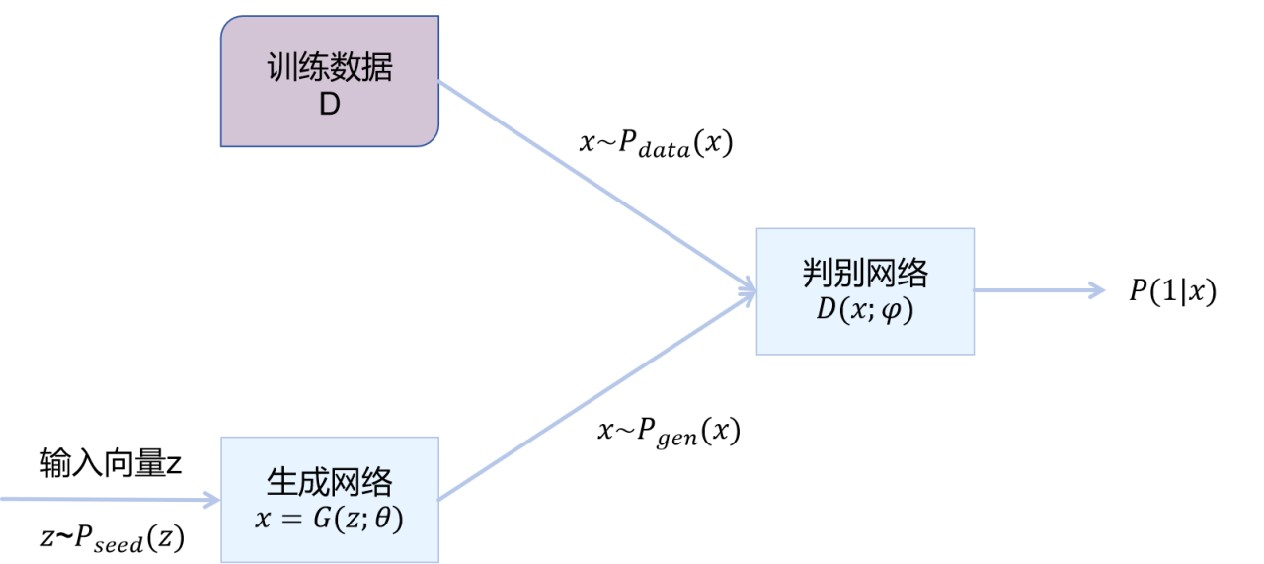
\includegraphics[width=10cm]{image/chap02/GAN.jpg}
    \caption{GAN的基础框架}
    \label{fig:GAN}
\end{figure}

判别网络和生成网络形成博弈关系,训练过程依赖与判别器的结果反馈,基于极大似然估计的思想,可以得到GAN的学习目标函数[附录补充]:
\begin{equation}
    \label{eq:example-formulas}
    V(G,D)=\underset{\theta}{\min}\underset{\phi}{\max}\Big[E_{x\sim P_{data}(x)}\log D(x;\phi)+E_{z\sim P_{seed}(z)}\log(1-D(G(z;\theta);\phi)]\Big]
\end{equation}

在GAN框架下,随着训练进行,生成器$G$生成图像质量越高,判别器$D$越可能误判,导致训练损失增加;判别器$D$判别能力越强,生成器$G$生成的图像更可能被打上“假”标签,训练损失增加。
最终两者在不断优化对抗下达到最优的对抗结果。在算法流程中,这种博弈关系体现为生成器与判别器交替进行神经网络的参数更新,参见\autoref{algo:GAN}。

\begin{algorithm}[h]
    \KwIn{训练集$\mathcal{D}$,对抗训练迭代次数$T$,每次判别网络的训练迭代次数$K$,小批量样本数量$M$}
    \For{$t\leftarrow 1$ \KwTo $T$}
    {
        //训练判别网络$D(x;\phi)$\\
        \For{$k\leftarrow 1$ \KwTo $K$}{
            //采集小批量训练样本\\
            从训练集$\mathcal{D}$中采集$M$个样本$\{x^{(m)}\},1\leq m\leq M$\\
            从分布$\mathcal{N}(\mathbf{0,I})$中采集$M$个样本$\{\mathbf{z}^{(m)},1\leq m\leq M\}$\\
            利用梯度下降法更新判别器网络参数
            \[
            \frac{\partial}{\partial \phi}\left[\frac{1}{M}\sum_{m=1}^M\left(log\ D(x^{(m)};\phi)+\log(1-D(G(z^{(m)};\theta);\phi))\right)\right]
            \]
        }
        //训练生成网络$G(z;\theta)$
        从分布$\mathcal{N}(\mathbf{0,I})$中采集$M$个样本$\{z^{(m)}\},1\leq m\leq M$\\
        利用梯度下降法更新生成器网络参数
        \[
        \frac{\partial}{\partial\theta}\left[\frac{1}{M}\sum_{m=1}^M D(G(z^{(m)};\theta),\phi)\right]
        \]
    }
    \KwOut{生成网络$G(z,\theta)$}
    \caption{生成对抗网络训练过程}
    \label{algo:GAN}
\end{algorithm}

\subsection{深度卷积生成对抗网络}
GAN的思想简单而深刻,在实际工程已有成熟的应用。本文实验主要基于一种广泛应用的GAN网络架构——深度生成对抗网络(Deep Convolutional GAN)。
DCGAN的研究成果\cite{radford2015unsupervised}发表于2015年。DCGAN基于GAN的思想,结合卷积神经网路,提出了全新的网络框架。DCGAN在训练中状态稳定,可以高质量地生成图片。并且展现了存在语义标签时,对图像生成结果的可控干扰。

DCGAN架构的设计规则主要聚焦于以下三点:

1)卷积层替代池化层:卷积神经网络(convolutional neural network)被证明可以有效捕捉图片特征,有助于网络下采样。

2)去除全连接层:减少网络参数量,尽可能避免过度对训练集的拟合,同时有助于加快网络训练速度

3)使用批归一化:批归一化(Batch normalization)对每一层的输入进行归一化处理,有效稳定数据分布。是一种加速训练并提高模型稳定性的技术。

\autoref{fig:DCGAN}展示了DCGAN中生成网络与判别网络架构。其中生成网络输入为长度100的潜在随机变量,而判别网络输出单一的判别结果。
\begin{figure}[!htbp]
    \centering
    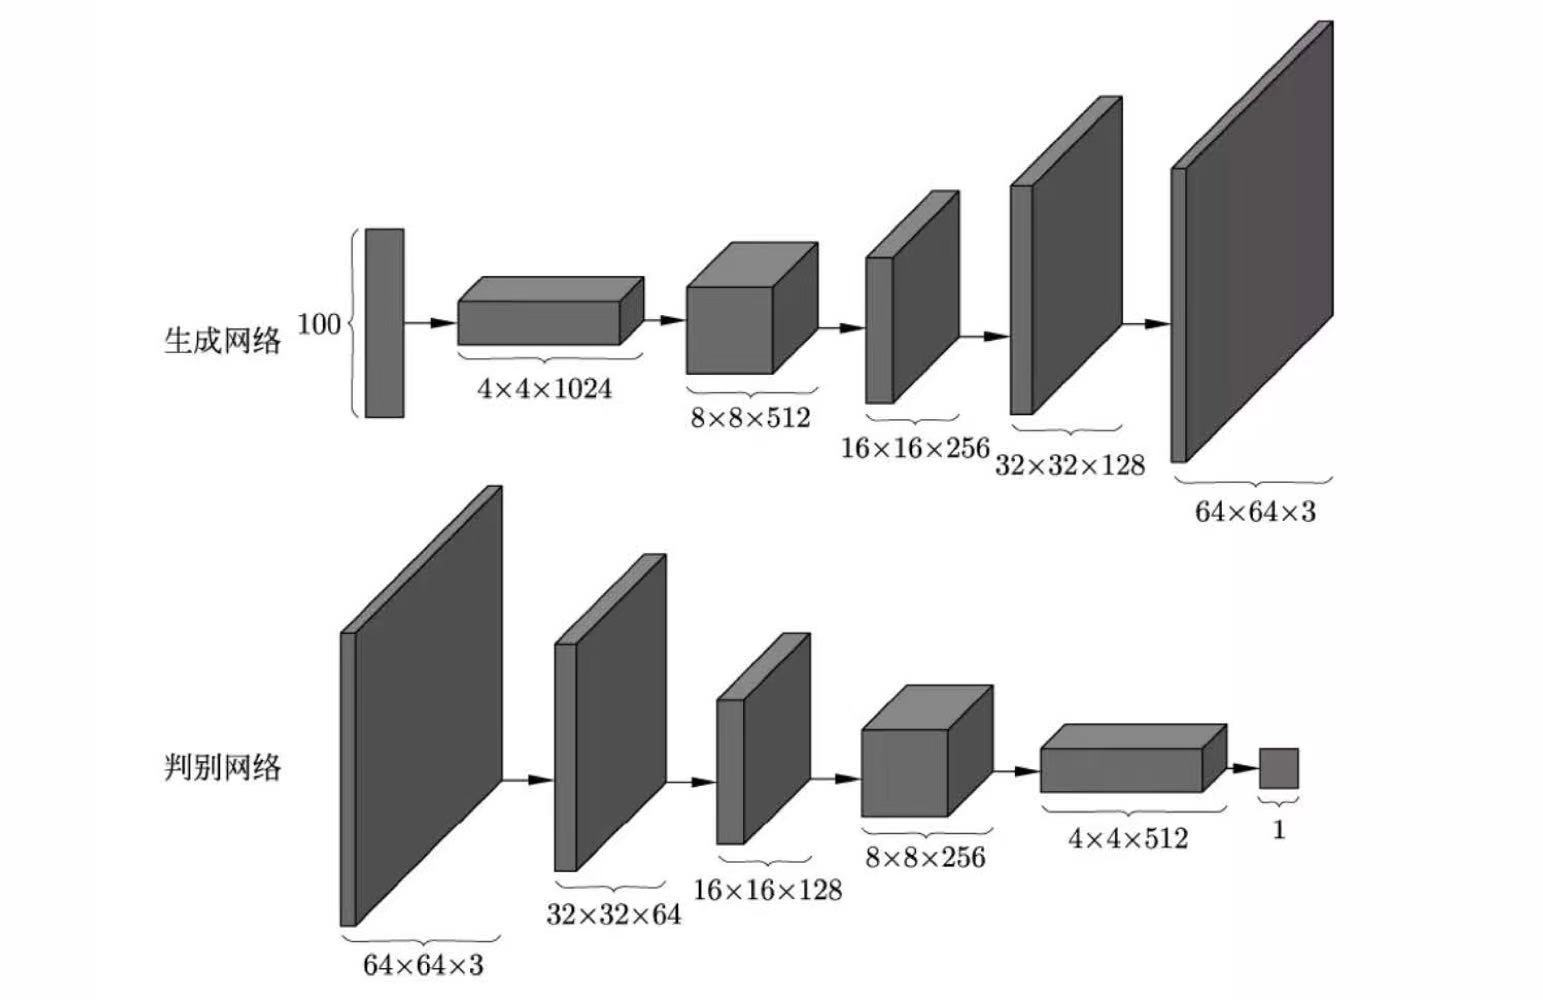
\includegraphics[width=10cm]{image/chap02/DCGAN.png}
    \caption{DCGAN网络结构}
    \label{fig:DCGAN}
\end{figure}

在实验中,生成对抗模型依然存在许多问题\cite{zhangtowards}。包括模式崩溃(生成器生成固定模式通过判别,生成样本失去多样性)、训练难度大(同时训练两个网络,存在多个超参数),解释性差(由于复杂博弈过程,图像生成过程缺乏解释性)。

\section{扩散模型}
扩散模型受热力学扩散过程的启发\cite{sohl2015deep},其目标是通过对数据点在潜空间中的扩散方式进行建模,来学习数据集的潜在结构。
扩散过程从数学角度来说就是:数据点的分布可以通过不断地添加噪声变成另一个分布。这种思路在图像生成任务中体现为:训练集的图像可以通过不断添加噪声,变成符合标准正态分布的图像(噪声)。
扩散模型通过神经网络学习添加噪声的过程,并可以实现加噪声的逆过程。在计算机视觉领域,这意味着可以通过学习逆扩散过程来训练神经网络,使其能对叠加了高斯噪声的图像进行去噪成像(从符合标准正态分布的噪声图像中去除噪声,得到图像)

扩散模型可以应用于各种任务,如图像去噪、图像修复、超分辨率成像、图像生成等等。Jonathan Ho等人在2020年论文《Denoising Diffusion Probabilistic Models》\cite{ho2020denoising}中利用扩散模型DDPM实现了高质量的图像生成,建立了前向加噪-反向降噪-训练的代码框架。
\subsection{前向过程}
在前向过程中,设定最大加噪次数的超参数$T$,对训练集的图像$x_0$添加$T$次噪声以使时刻$T$的图像$x_T$符合标准正态分布。
准确来说,\textbf{加噪声}并不是给$t-1$时刻的图像$\mathbf{x}_{t-1}$加上噪声值,而是从一个均值与图像$\mathbf{x}_{t-1}$相关的正态分布中采样新图像。
如\autoref{eq:sample}所示,$\mathbf{x}_{t-1}$是上一时刻的图像,$\mathbf{x}_t$是这一时刻生成的图像,该图像是从一个均值与$\mathbf{x}_{t-1}$有关的正态分布里采样出来的。
\begin{equation}
    \mathbf{x}_t\sim\mathcal{N}\Big(\mu_t(\mathbf{x}_{t-1}),\sigma_t^2\mathbf{I}\Big)
    \label{eq:sample}
\end{equation}
其中$x_t$只与上一时刻$x_{t-1}$有关,而与$x_{t-2},x_{t-3}...$无关,这说明前向过程是一个马尔科夫过程
\footnote{在概率论及统计学中,马尔可夫过程(Markov process)是一个具备了马可夫性质的随机过程,因为俄国数学家安德雷·马可夫得名。马尔可夫过程是不具备记忆特质的。换言之,马尔可夫过程的条件概率仅仅与系统的当前状态相关,而与它的过去历史或未来状态,都是独立、不相关的}。
这使得前向过程有良好的数学性质。
\begin{align*}
    \begin{split}
        q(x_1,...,x_T|x_0)=\prod_{t=1}^{T}q(x_t|x_{t-1})\\ 
        q(x_t|x_{t-1})=\mathcal{N}(x_t;\sqrt{1-\beta_t}x_{t-1},\beta_t\mathbf{I})
    \end{split}
\end{align*}

设置合适的加噪扩散次数$T$和具有特定性质的$\beta_t$,我们可以利用一步扩散公式得到从初始图像$x_0$得到任意时刻图像$x_t$的公式。详细推导可参考附录A
\begin{equation}
    x_t=\sqrt{\Pi_{i=1}^{t}(1-\beta_i)}x_0+\sqrt{1-\Pi_{i=1}^{t}(1-\beta_i)}
\end{equation}
为简化结果,令$\alpha_t=1-\beta_t,\overline{\alpha_t}=\prod_{i=1}^{t}\alpha_i$,可以得到$x_t$关于$x_0$的条件分布。
其中$1-\overline{\alpha_t}$反映了$t$时刻的此条件分布的方差。
\begin{equation}
    q(x_t|x_0)=\mathcal{N}(x_t;\sqrt{\bar{\alpha_t}},(1-\bar{\alpha_t})\mathbf{I})
\end{equation}

\subsection{反向过程}

正向过程设置了$T$步加噪声过程。在反向过程中,如果能够实现取消每一步加噪声操作,让一个纯噪声图像变成类似数据集的图像,就达到了图像生成的目标。
如何得到每一步的噪声,并且去除噪声,使得任意一个从标准正态分布里采样出来的噪声图像分布都能还原为训练集的图像分布。
扩散模型DDPM使用深度神经网络来预测每一步的噪声,并进行去噪声操作。数学原理表明[附录补充],当$\beta_t$足够小时,每一步加噪声的逆操作也满足正态分布。
\begin{equation}
    \mathbf{x}_{t-1}\sim\mathcal{N}(\tilde{\mu_t},\tilde{\beta_t}\mathbf{I})
\end{equation}
其中,当前时刻加噪声逆操作的均值$\tilde{\mu_t}$和方差$\tilde{\beta_t}$由当前时刻$t$,当前的图像$x_t$决定。
因此,为了描述所有去噪声操作,神经网络需要输入$t$,$x_t$,拟合前一步图像$\mathbf{x}_{t-1}$服从分布的均值$\tilde{\mu_t}$和方差$\tilde{\beta_t}$。

在理想情况下,去操作就等于加噪声操作的逆操作。DDPM模型使用神经网络拟合噪声,这反映\textbf{去噪声}和\textbf{加噪声逆操作}的关系
就是神经网络的\textbf{预测值}和\textbf{真值}的关系。从概率分布的角度来说就是,如何尽可能使条件分布$q(\mathbf{x}_t|\mathbf{x}_{t-1})$接近$p_{\theta}(\mathbf{x}_{t-1}|\mathbf{x}_t)$,参见\autoref{fig:DDPM}。
\begin{figure}[!htbp]
    \centering
    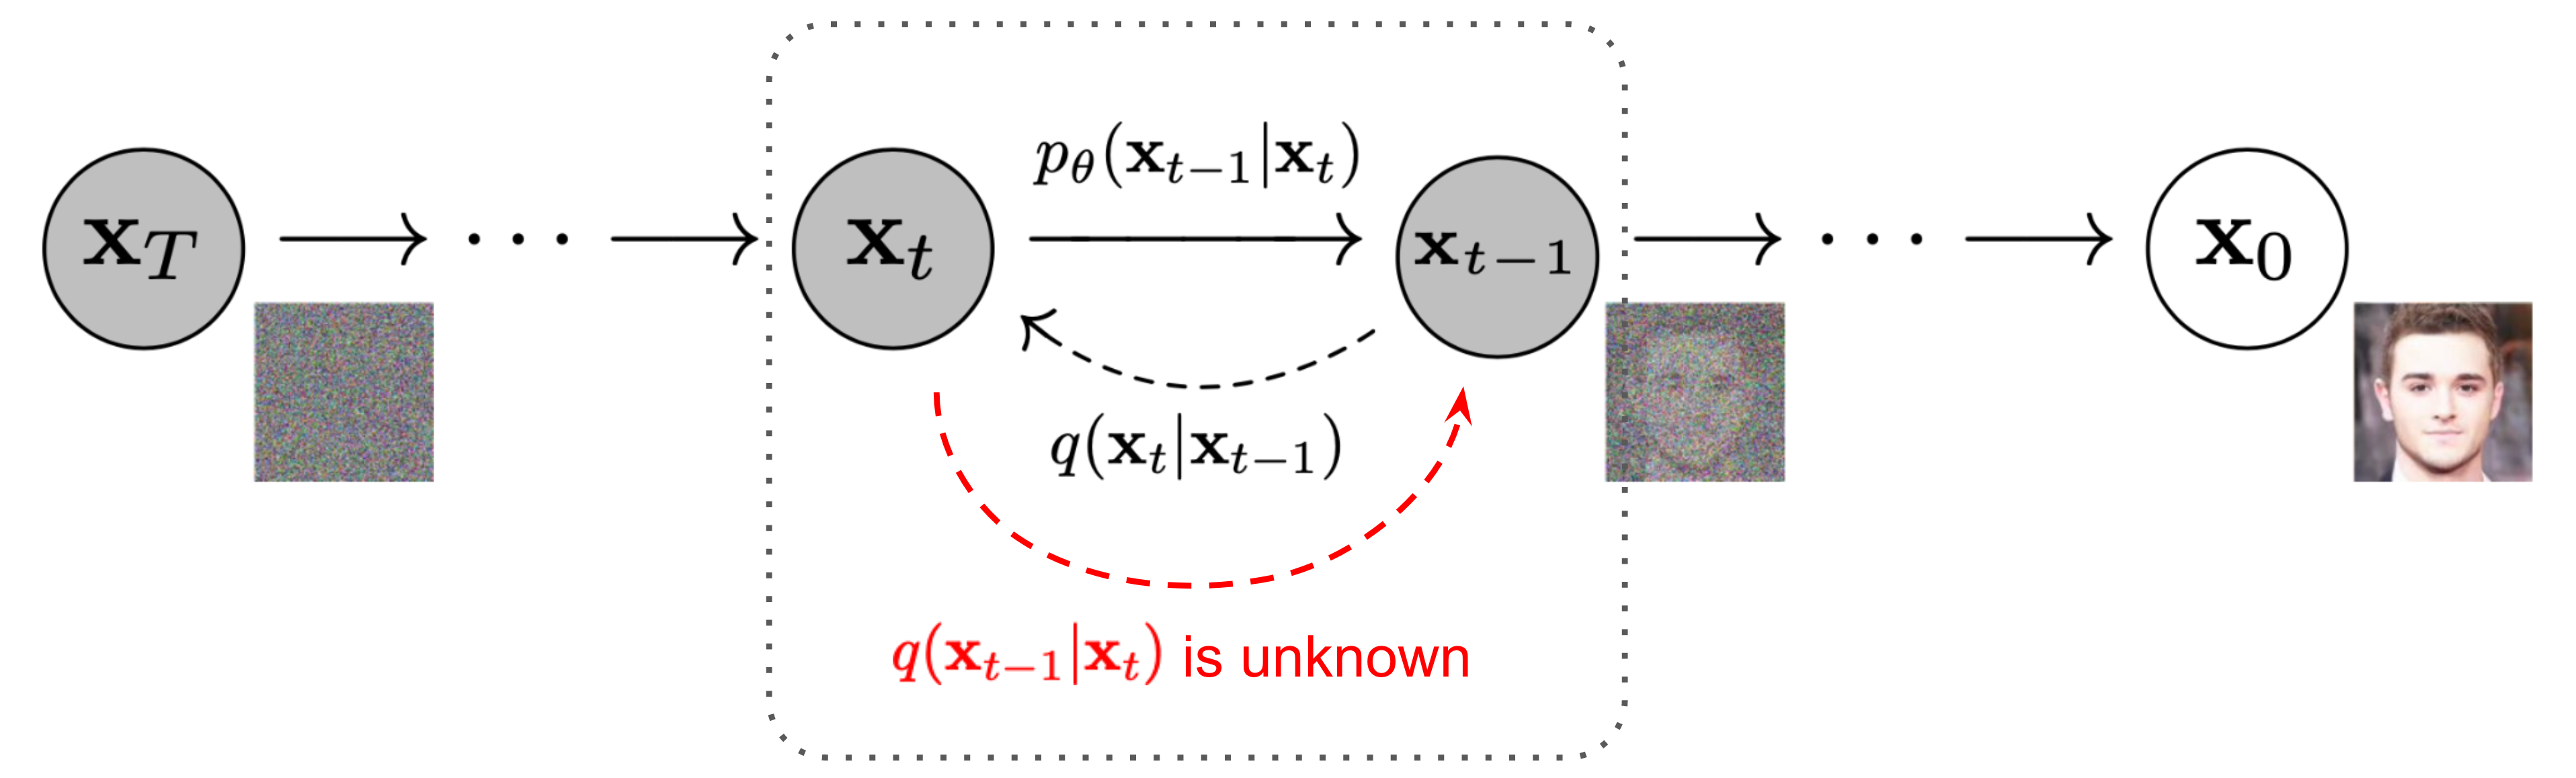
\includegraphics[width=10cm]{image/chap02/DDPM.png}
    \caption{DDPM示意图}
    \label{fig:DDPM}
\end{figure}
然而,直接计算所有数据的加噪声逆操作的分布是困难的。但若给定了训练集输入$x_0$,利用贝叶斯公式可以计算得到
$$
q(x_{t-1}|x_t,x_0)=q(x_t|x_{t-1},x_0)\dfrac{q(x_{t-1}|x_0)}{q(x_t|x_0)} 
$$
在上面的等式中,左边的$q(x_{t-1}|x_t,x_0)=\mathcal{N}(x_{t-1};\tilde{\mu_t},\tilde{\beta_t}\mathbf{I})$表示加噪声操作的逆操作,它的均值和方差都是待求的。
右边的$q(x_t|x_{t-1},x_0)=\mathcal{N}(x_t;\sqrt{1-\beta_t}x_{t-1},\beta_t\mathbf{I})$是加噪声的分布。
由于$\mathbf{x_0}$已知,$q(x_{t-1}|x_0)$和$q(x_t|x_0)$两项可以根据公式$x_t=\sqrt{\bar{\alpha_t}}x_0+\sqrt{1-\bar{\alpha_t}}\epsilon_t$得到:
\begin{equation}
    \begin{split}
        q(x_t|x_0)=\mathcal{N}(x_t;\sqrt{\bar{\alpha_t}}x_0,(1-\bar{\alpha_t})\mathbf{I}) \\
        q(x_{t-1}|x_0)=\mathcal{N}(x_{t-1};\sqrt{\bar{\alpha}_{t-1}}x_0,(1-\bar{\alpha}_{t-1})\mathbf{I})
    \end{split}
\end{equation}
这样等式右边的式子全部已知。将上式代入可以算出给定$x_0$时的去噪声分布。经计算[附录补充]化简,分布的均值$\tilde{\mu_t}$和方差$\tilde{\beta_t}$
\begin{equation}
    \label{eq:mean}
    \tilde{\mu_t}=\frac{1}{\sqrt{\alpha_t}}(x_t-\frac{1-\alpha_t}{\sqrt{1-\bar{\alpha_t}}}\epsilon_t)
\end{equation}
其中$\epsilon_t$是从标准正态分布采样处的样本。
\begin{equation}
    \tilde{\beta_t}=\frac{1-\bar{\alpha}_{t-1}}{1-\bar{\alpha_t}}\beta_t
\end{equation}
分布的方差与输入$x_0$无关,因此在训练神经网络进行去噪时,只需要拟合$T$步中各时刻均值即可,方差则由噪声方差$\beta_t$决定。
在利用去噪网络拟合均值时,参见\autoref{eq:mean},去噪过程中$\mathbf{x}_t$是已知的。唯一不确定是$\epsilon_t$。
所用设置的神经网络只需要预测噪声$\epsilon_{\theta}(\mathbf{x}_t,t)$(其中$\theta$为可学习参数)即可。

设置$\epsilon_{\theta}(\mathbf{x}_t,t)$和生成$\mathbf{x}_t$的噪声$\epsilon_t$的均方误差MSE最小即可。因此对于一轮训练,最终的损失函数可写成[附录补充]
\begin{equation}
    \mathbf{L}=\big|\big|\epsilon_t-\epsilon_{\theta}(x_t,t)\big|\big|^2
\end{equation}

\subsection{神经网络选择}
扩散模型DDPM的前向过程和反向过程,在算法流程中体现为训练神经网络\autoref{algo:train}和采样生成图像\autoref{algo:denoise}两部分。
\begin{algorithm}[h]
    \KwIn{训练集样本$x_0$}
    \While{损失函数未收敛到指定精度时}{
        \[
        t\sim\ Uniform(\{1,...,T\}),
        \epsilon\sim\mathcal{N}(\mathbf{0},\mathbf{I})
        \]
        利用梯度下降法更新去噪神经网络
        \[
        \nabla_{\theta}\big|\big|\epsilon-\epsilon_{\theta}(\sqrt{\bar{\alpha}_t}x_0+\sqrt{1-\bar{\alpha}_t\epsilon,t})\big|\big|^2
        \]
    }
    \caption{算法1:训练拟合噪声}
    \label{algo:train}
\end{algorithm}
在\autoref{algo:train}中,$\epsilon_{\theta}(x_t,t)$是一个神经网络的映射,输入图像$\mathbf{x}_t$和时间$t$输出噪声预测。
在DDPM中并没有规定神经网络要求,通常会根据图像生成任务的难易程度,定义简单或复杂的网络结构。
原始论文中\cite{ho2020denoising},所用神经网络是经典的U-Net网络
\footnote{U-Net最早是用于生物医学图像分割开发的卷积神经网络\cite{ronneberger2015u}。其基于完全卷积网络,并在结构上加以修改与扩展,使得它可以用更少的训练图像产生更精确的分割。
U-Net架构已经在扩散模型中采用,用于迭代式图像去噪音。该网络网络由一个收缩路径(contracting path)和一个扩展路径(expansive path)组成,使其具有U形结构。}。
\begin{algorithm}[h]
    \KwIn{噪声样本$x_T\sim\mathcal{N}(\mathbf{0},\mathbf{I})$}
    \For{$t=T,...,1$}{
        \[
        z\sim\mathcal{N}(\mathbf{0},\mathbf{I})if\ t>1,else\ z=0 
        \]
        \[
        x_{t-1}=\frac{1}{\sqrt{\alpha_t}}\left(x_t-\frac{1-\alpha_t}{\sqrt{1-\bar{\alpha_t}}}\epsilon_{\theta}(x_t,t)+\sigma_t\ Z\right)
        \]
    }
    \KwOut{拟合训练集的生成图像$\hat{x_0}$}
    \caption{算法2:去噪声生成图像过程}
    \label{algo:denoise}
\end{algorithm}

训练结束后,可以利用去噪声算法生成图像。由于$x_T$是从标准正态分布里随机采样的输入噪声,可以通过选取不同初始噪声,得到不同的图像生成结果,满足图像多样性的需求。